\title{UnisensViewer\\[0.5em]\Large User Documentation}
\author{Kristina Schaaff, Malte Kirst, Marcus Warga}
\maketitle
\tableofcontents

	\section{Application Area}
	
UnisensViewer has been developed for easy handling of multi sensor data stored in the Unisens data format \cite{Kirst2008,Unisens2008} directly after the recording as well as for data visualization. The workflow is simplified by a software-based solution for editing and creating of meta data for data sets. This meta data is stored in the Unisens data format. Moreover, UnisensViewer allows to easily edit measurement data. Additionally, the user interface can be used to display information about selected measurement data as well as annotations. Visualization of multiple sensor data can be done synchronous and in parallel. 


	\section{Installation}

UnisensViewer is an application for Windows XP, Windows Vista and Windows 7. If not already installed, the .Net-Framework 4.0 or higher has to be installed. Some systems additionally require installation of \textsl{Microsoft Visual C++ 2010 Redistributable Package}. Both packages are available at the Microsoft homepage \cite{Microsoft2010}.

The content of the zip-file has to be unpacked to a folder of your choice. The file \texttt{UnisensViewer.exe} can be executed immediately and will start the UnisensViewer.  




	\section{Structure of UnisensViewer}

UnisensViewer (see Figure \ref{fig:viewer}) consists of three areas: the menu bar (upper side), the sidebar at the left side and the display area at the right side. 

\begin{figure}[ht]
  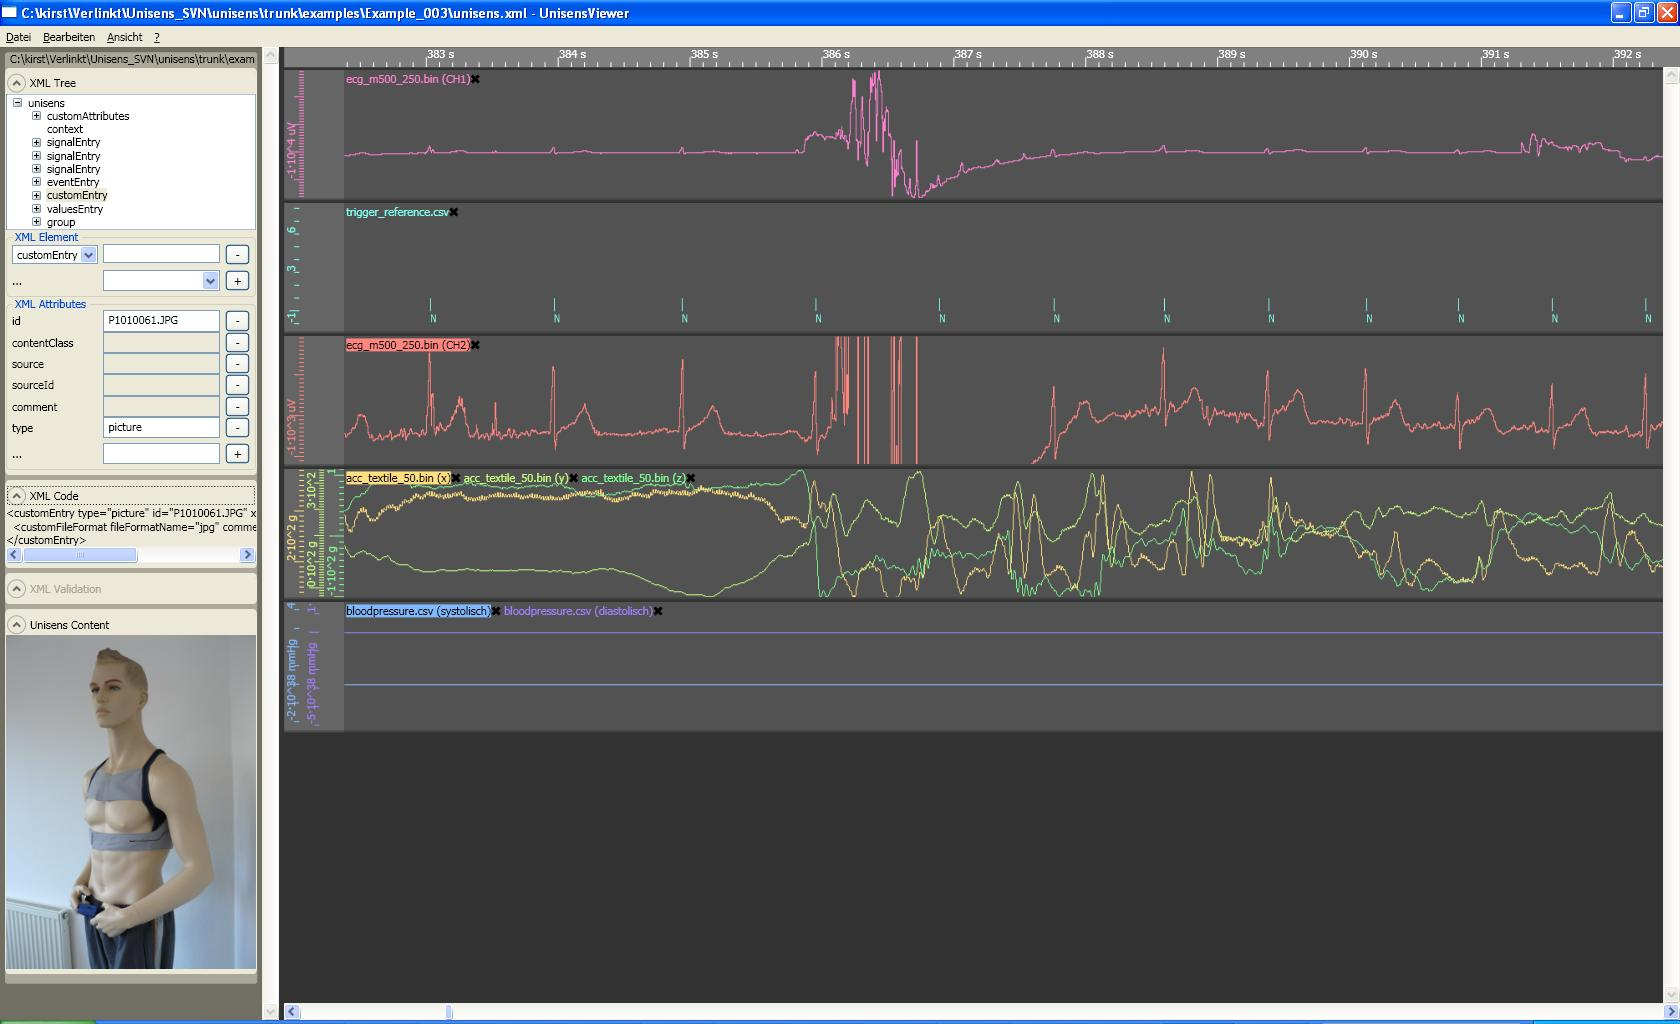
\includegraphics[width=\textwidth]{ressourcen/UnisensViewer.JPG}  	
	\caption{UnisensViewer: sidebar at the left side, display area on the right}
	\label{fig:viewer}
\end{figure}



		\subsection{Menu Bar}
		
The menu bar at the upper side of the window consists of the following items: 

\begin{description}
	\item[File] Open and save data sets and create new data sets
	\item[Edit] Not implemented yet
	\item[View] Functions for automatic zooming
	\item[Plug-ins] For installed plug-ins
	\item[?] Information about UnisensViewer
\end{description}



		\subsection{Sidebar}
	
The sidebar contains all (context) information from the \texttt{unisens.xml}. The width of the sidebar may be varied by dragging it with the mouse. 

Within the sidebar you will find various windows. The upper area contains cursor information displaying the time- and amplitude information of the current cursor position. If a signal part is marked with the mouse, further information about the marked area appears. 

The XML tree displays the meta information from the \texttt{unisens.xml} in a tree structure. It is possible to browse this tree by klicking at the elements to fold or unfold the elements. For the selected element all corresponding attributes are shown at the sidebar. 


The code view (\textsl{XML Code}) shows the area of the \texttt{unisens.xml} which is marked in the XML tree. 

The validation view  (\textsl{XML Validation}) shows the information of the integrated XML validator. If the \texttt{unisens.xml} is not conform to the associated XSD (XML Schema Document), errors are shown in this view. 

The content view (\textsl{Unisens Content}) contains selected contents of a data set. This can for instance be the content of the \texttt{context.xml} or a CustomEntry. 



		\subsection{Display Area}
		
The display area shows signals, measurement values and annotations. Mouse gestures can be used for zooming and scrolling. The data displayed can be moved and / or stacked by drop \& drag. 


	\section{Using the UnisensViewer}

The file \texttt{UnisensViewer.exe} can be executed immediately and will start the program. This section describes the usage of the Viewer. Main features are the support of mouse gestures, drag \& drop and the context menu.


		\subsection{Opening Data Files}
		
Data files can be opened using the open file dialog (\textsl{File} \textrightarrow\ \textsl{Open...} or \textsf{Ctrl} + \textsf{o}) or by drop \& drag of the file into the XML tree. Subsequently, the data set will appear in the XML tree. 


		\subsection{Displaying Signals, Measured Data and Annotations}

To display signals, measured data and annotations, the corresponding entry (SignalEntry, ValuesEntry or EventEntry) has to be dragged from the XML tree to the display area. Each entry can only be displayed once in the display area. All elements include a name tag in the format \textsl{EntryId (ChannelName)}. The displayed elements can be resorted by drag \& drop, stapled, or unstapled. The area which is sensitive for drag \& drop is the name tag of the corresponding element. 


		\subsection{Using the XML Editor}

The XML editor which is integrated in the sidebar is responsible to view, edit or create the files \texttt{unisens.xml} and \texttt{context.xml}. 
	
	
	
		\subsection{Display of CustomEntries}
		
Context information can be chosen from the XML tree, it is displayed in the lower area (\textsl{Unisens Content}) of the sidebar. Until now, the following data formats are supported: 
	
\begin{table}[ht]
	\caption{Supported context information}
	\begin{tabularx}{\textwidth}{lX}
		\hline
		file extension & description \\
		\hline
		\hline
		JPG & picture preview \\
		PNG & picture preview \\
		\hline
	\end{tabularx}
	\label{tab:contentclass}
\end{table}
	\[
\]



		\subsection{Horizontal and Vertical Zooming / Scaling}
Zooming and scaling of the displayed signals is done by mouse gestures. Horizontal zooming (time axis) includes all displayed signals. Vertical zooming / scaling includes all chosen signals of the current stack. Signals can be chosen by klicking on the name tag. 

\begin{description}
	\item[Horizontal zooming] middle mouse button + vertical mouse gesture, Alt + middle mouse button + vertical mouse gesture or Alt + left mouse button + vertical mouse gesture
 	\item[Vertical zooming] shift + middle mouse button + horizontal mouse gesture
\end{description}



		\subsection{Moving and Scrolling}
Moving and scrolling of signals is done by mouse gestures or by the horizontal scroll bar at the lower side of the display. Horizontal scrolling (time axis) includes all displayed signals. Vertical scrolling refers to all selected signals of the current stack. Signals can be chosen by their name tag. 


\begin{description}
	\item[Horizontal scrolling] middle mouse button + horizontal mouse gesture, Alt + middle mouse button + horizontal mouse gesture, Alt + left mouse button + horizontal mouse gesture, or by using the scroll bar
	\item[Vertical scrolling] Ctrl + middle mouse button + vertical mouse gesture
\end{description}

By pressing Ctrl + Shift at the same time, gestures for vertical scrolling and vertical zooming can be combined. 




		\subsection{Automatic Scaling}
		
Signals can be scaled automatically. For automatic scaling \textsl{Auto scale} has to be selected from the context menu (for the current stack or the selected signals of the current stack). To scale all displayed signals, select \textsl{View} \textrightarrow\ \textsl{Auto scale} from the menu bar and select the preferred scaling function. The following scaling options are supported: 


\begin{description}
	\item[Distinct signals] Signals are scaled such that each signal fully uses the available space. 
	\item[Grouped by files] Signals are grouped before scaling, all files belonging to one entry belong to one group. These signals are scaled around zero with the same factor such that the space at the display is fully used. 
	\item[Grouped by units] Before scaling, signals are grouped, all data files with the same physical dimension belong to the same group. These signals are scaled with the same factor around zero such that the display space is fully used. 
\end{description}



	\subsection{Create New Data Sets}
	
To create a new data set, select \textsl{File} \textrightarrow\ \textsl{New} from the menu or press Ctrl + N. Subsequently, the elements from tre XML tree have to be selected. Next the required attributes can be filled in using the editor. The Unisens data set can then be stored at a folder of your choice. 

Entries can be added to the data set by putting them per drag \& drop to the XML tree. The files have to be locaed in the same folder like the \texttt{unisens.xml} (otherwise data set cannot be opened later). \texttt{bin} files are automatically added as a SignalEntry while \texttt{csv} files are added as EventEntry. 


	\section{Plug-Ins}
	
	\subsection{Installation}
	
It is possible to extend the UnisensViewer by plug-ins. The installation of plug-ins is done by copying the plug-in file into the folder \textsl{Plugins}. After the next start fo the UnisensViewer, the plug-in appears in the corresponding menu. 



	\subsection{Using Plug-Ins}
	
A plug in can - depending on the kind of the plugin - be used for single or multiple entries. 


	\section{License}

UnisensViewer is a development of FZI Forschungszentrum Informatik. The software is provided "as is", without warranty of any kind, express or implied, including but not limited to the warranties of merchantability, fitness for a particular purpose and noninfringement. In no event shall the consortium be liable for any claim, damages or other liability, whether in an action of contract, tort or otherwise, arising from, out of or in connection with the software or the use or other dealings in the software.

If you use Unisens for scientific research, please refer to the Unisens data format and the Unisens homepage  \texttt{http://www.unisens.org} \cite{Unisens2008} in your publications. 

The Unisens library and the Unisens interface are licensed under GNU Lesser General Public License (LGPL). The license text is delivered together with the code and can be found at \cite{lgpl2008}. You can get the Unisens libary and the Unisens interface at the Unisens project homepage \texttt{http://www.unisens.org}.



%%%%%%%%%%%%%%%%%%%%%%%%%%%%%%%%%%%%%%%%%%%%%%%%%%%%%%%%%%%%%%%%%%%%%%%%%%%%%%%%%%%%
%
%  Literaturverzeichnis
%
%%%%%%%%%%%%%%%%%%%%%%%%%%%%%%%%%%%%%%%%%%%%%%%%%%%%%%%%%%%%%%%%%%%%%%%%%%%%%%%%%%%%


\bibliographystyle{mit_din}
\bibliography{Unisens}

%XML
%XSD
%CSV Format
%Floating Point Spec
%FAT16: http://de.wikipedia.org/wiki/File_Allocation_Table#FAT16
%WFDB Format: http://www.physionet.org/physiotools/wpg/wpg.htm
%\nocite{moody2008}


%%%%%%%%%%%%%%%%%%%%%%%%%%%%%%%%%%%%%%%%%%%%%%%%%%%%%%%%%%%%%%%%%%%%%%%%%%%%%%%%%%%%
%
%  Kontakt
%
%%%%%%%%%%%%%%%%%%%%%%%%%%%%%%%%%%%%%%%%%%%%%%%%%%%%%%%%%%%%%%%%%%%%%%%%%%%%%%%%%%%%

	\section*{Contact}

\paragraph{FZI Forschungszentrum Informatik} ~\\
Embedded Systems and Sensors Engineering (ESS)\\
Haid-und-Neu-Str. 10--14\\
76131 Karlsruhe\\
Germany\\[1ex]
Dipl.-Ing. Malte Kirst\\
kirst@fzi.de

\paragraph{Universit�t Karlsruhe} ~\\
Institut f�r Technik der Informationsverarbeitung (ITIV)\\
Engesserstr. 5\\
76131 Karlsruhe\\
Germany\\[1ex]
Dipl.-Ing. J�rg Ottenbacher\\
ottenbacher@itiv.uni-karlsruhe.de

\paragraph{http://www.unisens.org}
